With the results found in this paper, we have accurately described what kind of behavior is present about the non-smooth bifurcation when new mechanisms are introduced in both the one-dimensional model \eqref{eq:oneD_canonical} and two-dimensional Stommel model \eqref{eq:twoD_canonical}. We had considered the mixture of early bifurcation due to high oscillatory forcing $\Omega\gg 1$ with amplitude $A\sim O(1)$ and the delayed tipping due to slow variation in the bifurcating parameter at rate $\epsilon\ll 1$. The main result being that these mechanisms have opposite effects on the tipping point and do mix with a kind of weighted average to produce an effective tipping approximation. These results give insight into the hysteresis behavior of the Stommel model and the understudied realm of non-smooth dynamics. The main approach used asymptotic expansions as well as the methods of multiple scales to identify reduced equations and find asymptotic solutions to the systems of differential equations. We found that depending on the region and mechanism, the reduced equations have differing expressions depending on the size of the solution. We also discover that linking the slow variation $\epsilon$ and the frequency $\Omega$ gives important insight into how the system will behave. 

The method developed in the one-dimensional model was to find an outer asymptotic expansion by separating the order of dynamics by a common small value, typically in terms of $\epsilon$. With the outer dynamics explicitly written, we scaled the model to find the inner equations to a reduced problem. From the inner equations, we solve and determine when the solution is no longer controllable. This resulted in the tipping points/bifurcations in the one-dimensional system \eqref{eq:oneD_canonical} which had good agreement with the numerical results from a simple differential equation solver. Due to the many similarities to the two-dimensional system \eqref{eq:twoD_canonical} we were able to modify the same analysis to find the tipping/bifurcations here as well.

Although the work here is not entirely finished where an analysis would need to be done on cases where $\Omega\sim O(1)$ or smaller. This case functions qualitatively different as slow oscillations have more contribution to the dynamics. This is also seen from the analysis where low frequency oscillations no longer allow for asymptotic expansions in terms of $\Omega^{-1}$ and no longer fall under our assumptions to integrate with $T_1$ and $T_2$. Thus this case behaves fundamentally different and can influence tipping in a way we hadn't explored here. This is shown in figure~\ref{fig:low_freq}. Also, large amplitude behavior $A\gg 1$ can force an additional rescaling before any familiar approaches hold. This is seen in figure~\ref{fig:large_amp}. These cases were mentioned but have yet to be performed on this model, although both have been studied around the smooth case in \cite{zhu2015tipping}. It is possible that they could have some surprising results in the non-smooth case. These cases would help further classify the tipping behavior for the variety of cases in real world ocean dynamics.

\begin{figure}[H]
\centering
\begin{subfigure}{.5\textwidth}
 \centering
 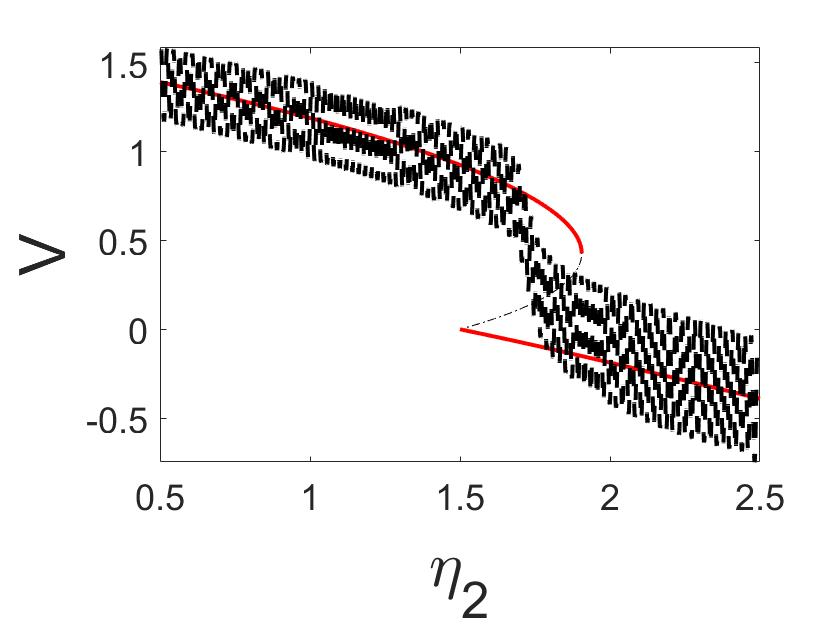
\includegraphics[width=\linewidth]{conclusion/low_freq_V.jpg}
 \caption{}
\end{subfigure}%
\begin{subfigure}{.5\textwidth}
 \centering
 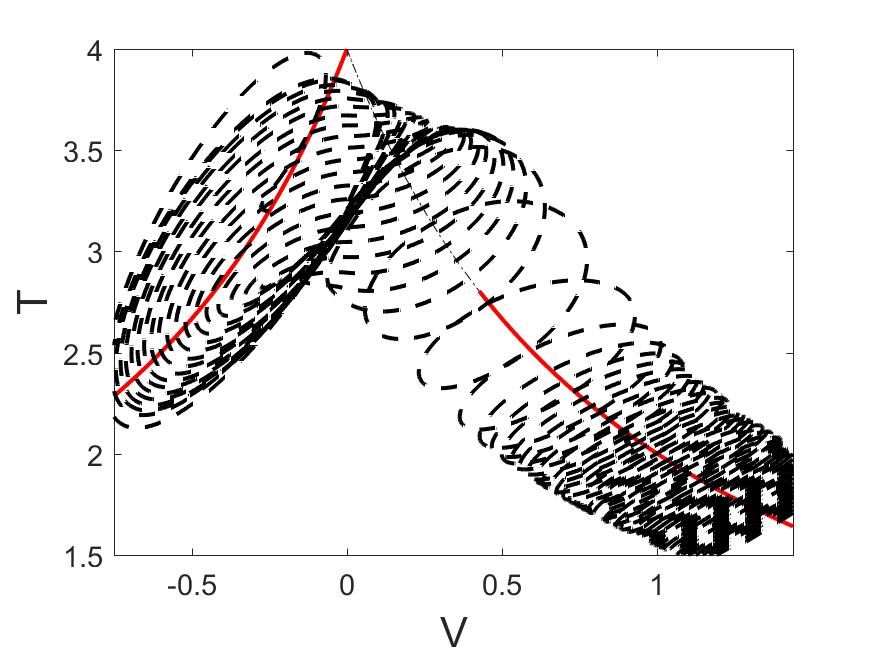
\includegraphics[width=\linewidth]{conclusion/low_freq_T.jpg}
 \caption{}
\end{subfigure}
\caption{Low Frequency: Model parameters are $\epsilon=.01$, $A=B=1$ and $\Omega=3$.}
\label{fig:low_freq}
\end{figure}

\begin{figure}[H]
\centering
\begin{subfigure}{.5\textwidth}
 \centering
 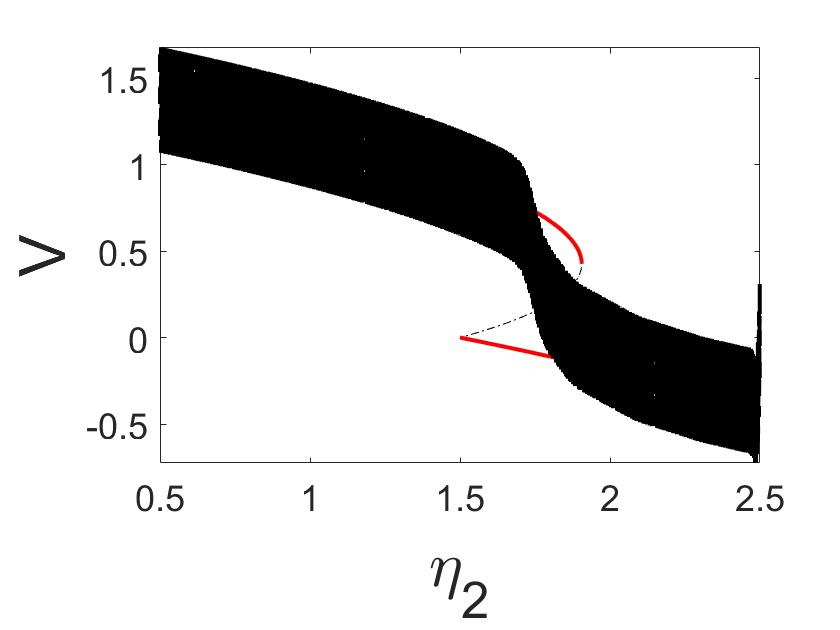
\includegraphics[width=\linewidth]{conclusion/large_amp_V.jpg}
 \caption{}
\end{subfigure}%
\begin{subfigure}{.5\textwidth}
 \centering
 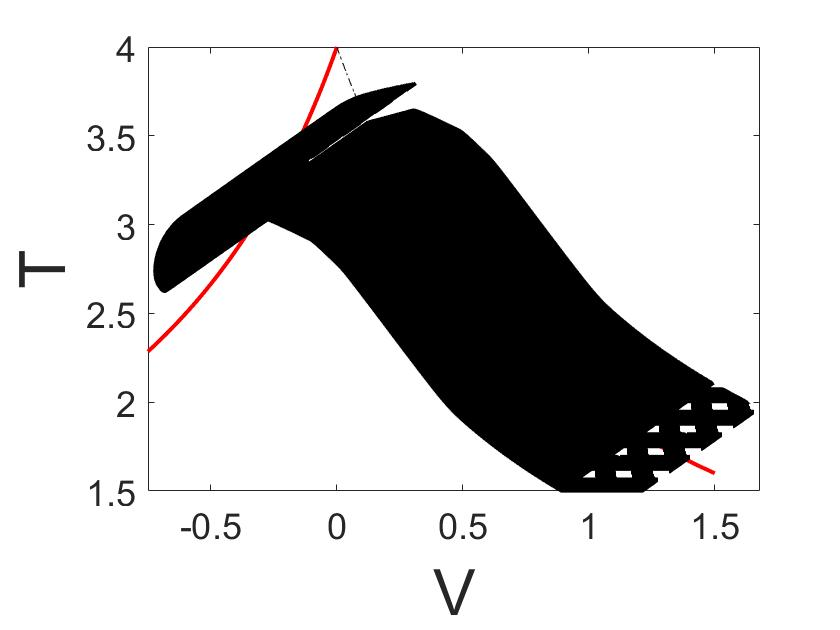
\includegraphics[width=\linewidth]{conclusion/large_amp_T.jpg}
 \caption{}
\end{subfigure}
\caption{Large Amplitude: Model parameters are $\epsilon=.01$, $A=B=300$ and $\Omega=1000$.}
\label{fig:large_amp}
\end{figure}

Lastly, we considered all deterministic behavior throughout this analysis but there are many reasons to incorporate stochastic elements into the Stommel model as well, see \cite{lorenzo2012role}. From \cite{zhu2015tipping} it is concluded that stochastic forcing has elements of both early bifurcations and delayed tipping and thus a natural follow-up to the analysis in this paper. We could consider stochastic forcing with

\begin{equation}\label{eq:stochastic}
\begin{aligned}
\dot{V} & = \eta_1-\eta_2+\eta_3(T-V)-T-V|V|+A\xi_1(t), \\
  \dot{T}   & = \eta_1-T(1+|V|)+B\xi_2(t), \\
 \dot{\eta_2} & = -\epsilon\\
 V(0)=&V^0,\quad T(0)=T^0, \quad \eta_2(0)={\eta_2}^0,
\end{aligned}
\end{equation}

where $\xi_i(t)$ is standard Gaussian noise with mean 0 and variance $t$ and initial conditions centered on the lower branch. This is shown in figure~\ref{fig:stochastic} and it is clear a completely separate analysis is needed.

\begin{figure}[H]
\centering
\begin{subfigure}{.5\textwidth}
 \centering
 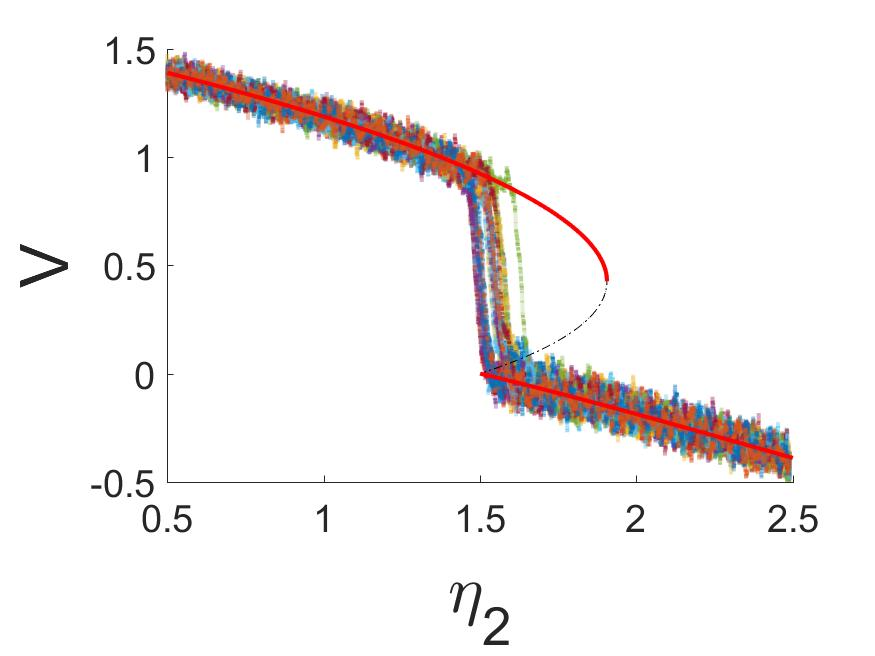
\includegraphics[width=\linewidth]{conclusion/stochastic_V.jpg}
 \caption{}
\end{subfigure}%
\begin{subfigure}{.5\textwidth}
 \centering
 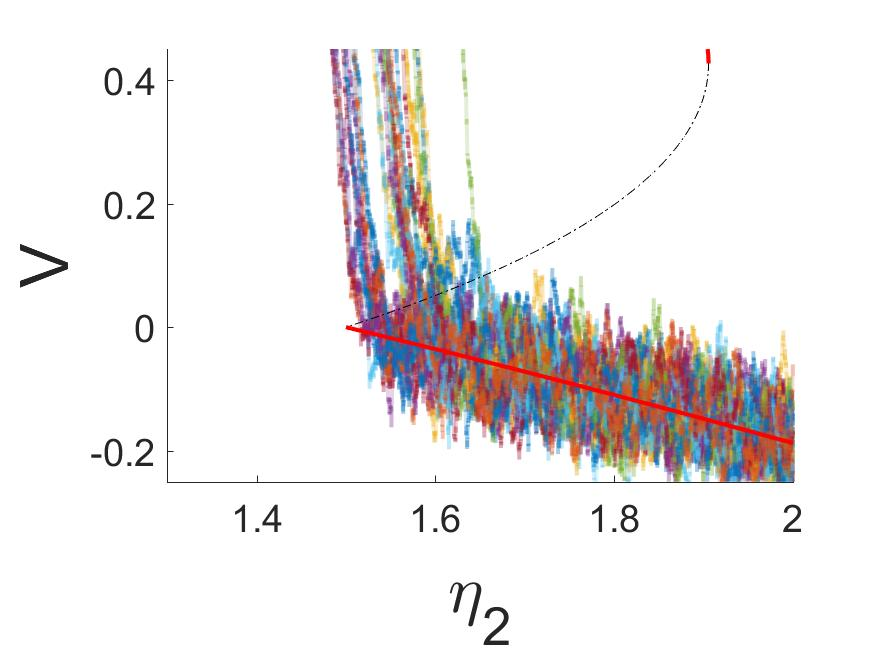
\includegraphics[width=\linewidth]{conclusion/stochastic_V_zoom.jpg}
 \caption{}
\end{subfigure}
\begin{subfigure}{.5\textwidth}
 \centering
 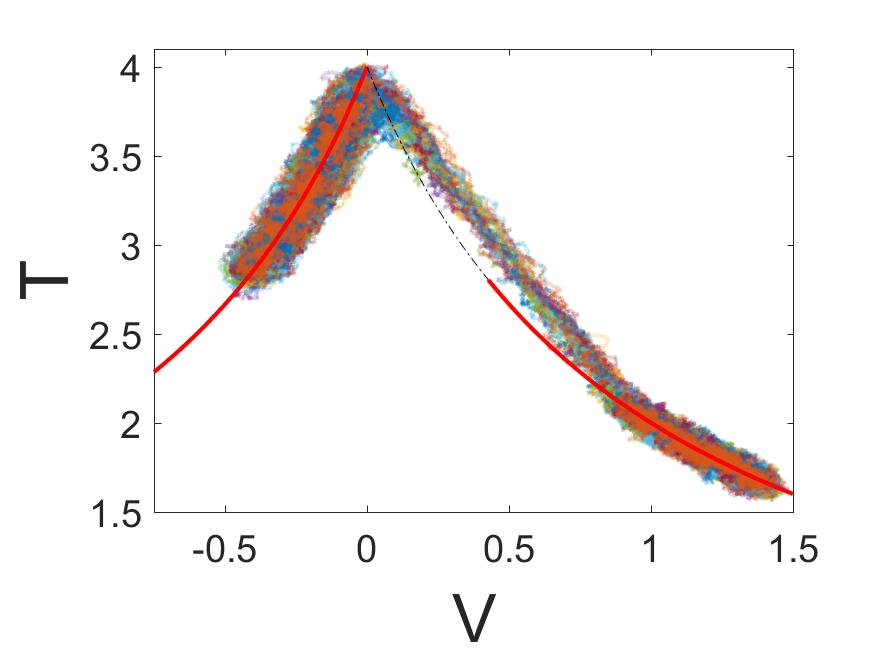
\includegraphics[width=\linewidth]{conclusion/stochastic_T.jpg}
 \caption{}
\end{subfigure}%
\begin{subfigure}{.5\textwidth}
 \centering
 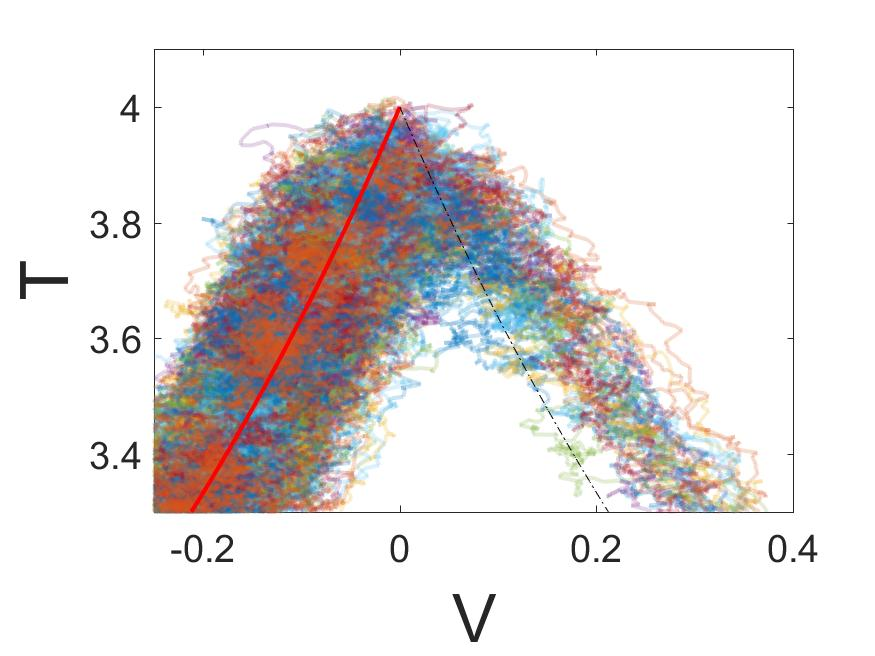
\includegraphics[width=\linewidth]{conclusion/stochastic_T_zoom.jpg}
 \caption{}
\end{subfigure}
\caption{Stochastic: In (a) many realizations of the numerical solution for $V$ in \eqref{eq:stochastic} is given with model parameters $\eta_1=4$, $\eta_3=.375$, $\epsilon=.01$ and $A=B=.7$. In (b) a zoom in closer to the non-smooth bifurcation region. In (c) we have the realizations over the standard equilibrium plot for $V$ vs. $T$. In (d) a zoom of the bifurcation area.}
\label{fig:stochastic}
\end{figure}